\documentclass[10pt, a4paper]{article}
\usepackage[T1]{fontenc}
\usepackage[utf8x]{inputenc}
\usepackage{ifpdf}
\usepackage{graphicx}
\usepackage{array}
\usepackage{multirow}


\usepackage{listings}	% For program listings.
\usepackage{color}
\definecolor{dkgreen}{rgb}{0,0.6,0}
\definecolor{gray}{rgb}{0.5,0.5,0.5}
\definecolor{mauve}{rgb}{0.58,0,0.82}
\lstset {
	language=Matlab,			  		% The language of the code.
	basicstyle=\footnotesize,			% The size of the fonts that are used for the code.
	numbers=left,						% Where to put the line-numbers.
	numberstyle=\tiny\color{gray},		% The style that is used for the line-numbers.
	stepnumber=1,						% The step between two line-numbers. If it's 1, each line will be numbered.
	numbersep=5pt,						% How far the line-numbers are from the code.
	backgroundcolor=\color{white},		% Choose the background color. You must add \usepackage{color}.
	showspaces=false,					% Show spaces adding particular underscores.
	showstringspaces=false,				% Underline spaces within strings.
	showtabs=false,						% Show tabs within strings adding particular underscores.
	frame=single,						% Adds a frame around the code.
	rulecolor=\color{black},			% If not set, the frame-color may be changed on line-breaks within not-black text (e.g. commens (green here)).
	tabsize=2,							% Sets default tabsize to 2 spaces.
	captionpos=t,						% Sets the caption-position to bottom.
	breaklines=true,					% Sets automatic line breaking.
	breakatwhitespace=false,			% Sets if automatic breaks should only happen at whitespace.
	title=\lstname,						% Show the filename of files included with \lstinputlisting;  also try caption instead of title.
	keywordstyle=\color{blue},			% Keyword style.
	commentstyle=\color{dkgreen},		% Comment style.
	stringstyle=\color{mauve},		  	% String literal style.
	escapeinside={\%*}{*)},			  	% If you want to add a comment within your code.
	morekeywords={*,...}			  	% If you want to add more keywords to the set.
}

\newcommand{\matlab}{\small{\emph{MATLAB\textsuperscript{\textregistered}}}}

\title{Numerical Analysis for Computer Scientists\\ FMN011, Lund University 2012\\ Project \#1\\ Solving huge systems of equations}
\date{}
\author{Erik Westrup, \texttt{<ada09ewe@student.lu.se>}}

\begin{document}
\begin{titlepage}
\maketitle

\thispagestyle{empty}
\end{titlepage}
\setcounter{page}{2}

\section{Introduction and Problem Background}
This project is about solving systems of very huge matrices. More specifically the matrices are not only huge but also almost banded and sparse which have important consequences and applications. A sparse quadratic $n\times n$  matrix is a matrix where the number of non-zero elements is, using big O notation, only $O(n)$ compared to a ``full'' matrix which has $O(n^2)$ non-zero elements. This is actually a common situation when we have measured information from the real world where not all the variables are depended on each other. To further explore the sparse system two types of methods for solving will be used: direct and iterative. Direct methods finds exact solution in a finite number of steps and iterative approaches the solution and finds and approximation only. The direct methods are useful when an exact solution is required (and exists) while iterative methods suits real time problem where data must be processed and close but not exact solution is sufficient. It is not always certain that iterative methods actually will converge towards the correct solution. However we will here only work with one specific sparse matrix for which we know an iterative method will converge.

In theory we can solve any large system (if it converge in the iterative case of course) but that requires equally much time. Unlimited computational power is (at present to be optimistic) not available and we have to deal with constraints in both time and memory. That is why we need to look at this problem from a computational point of view. Of course it's possible to theoretically consider the hardware specifications and analyze the execution of machine code to find out how large system we can solve. However it is much pragmatic and simpler to just test it on the hardware directly. So that is what will be done in this project.

The sparse $n \times n$ matrix A that should be used in this project is defined by:
\begin{eqnarray} \label{matrix+a}
		A(i,i-1)   & =	-1, & i\in[2,n] \nonumber \\
		A(i,i)	   & =	3, & i\in[1,n] \nonumber \\
		A(i,i+1)   & =	-1, & i\in[1,n-1] \nonumber \\
		A(i,n+1-i) & =	\frac{1}{2}, & i\in[1,n-1]\backslash \frac{n}{2}\wedge\frac{n}{2}+1
\end{eqnarray}

With $n=8$ it looks like this:
\begin{displaymath}
A = \left( \begin{array}{cccccccc}
  3   & -1  & 0   & 0  & 0  & 0   & 0   & 0.5 \\
  -1  & 3   & -1  & 0  & 0  & 0   & 0.5 & 0   \\
  0   & -1  & 3   & -1 & 0  & 0.5 & 0   & 0   \\
  0   & 0   & -1  & 3  & -1 & 0   & 0   & 0   \\
  0   & 0   & 0   & -1 & 3  & -1  & 0   & 0   \\
  0   & 0   & 0.5 & 0  & -1 & 3   & -1  & 0   \\
  0   & 0.5 & 0   & 0  & 0  & -1  & 3   & -1  \\
  0.5 & 0   & 0   & 0  & 0  & 0   & -1  & 3
\end{array} \right)
\end{displaymath}

\section{Numerical Considerations}
Exploiting the vacuity of a matrix in when it's used in numerical calculations gives great benefits since we only need to store the non-zero elements which saves us a factor of $O(n)$ in space which is important since a computer is limited in memory. Also matrix operations can be specialized that takes advantage of this structure to do less operations \cite{sparsemat}.

The most common direct method is the \emph{Gaussian elimination}\footnote{GE from now on.} and therefor it will be tested here \cite{gauss}. There are many iterative methods like Jacobi or Gauss-Seidel but we will here use a method called \emph{Successive Over-Relacation}\footnote{SOR from now on.} that is a modification of Gauss-Seidel that iterates more aggressively to achieve faster convergence. When the convergence is guaranteed we can iterative a given number of times, let it run for a given time or if we know the real solution until the maximum error is below some small $\epsilon.$ \cite{sor}.

To solve this any programming language could have been used but using tool and language developed for numerical computation makes the task much simpler. Thus I've used \matlab{} to implement and test the algorithms. \matlab{} have built in support for dealing with sparse matrices and most matrix operations are overloaded to exploit this as well. I've used many other features \matlab{} offers that does not affect the complexity but makes the code easier or more reusable including functions, packages, exceptions, formatted strings, default arguments and time measurements.

\subsection{Time out}
I wanted to run the script in a predetermined time since my computer is a shared resource that I need for a lot of other things. Also it is good to be able to run different tests the same amount of time one can make comparisons. It's not as simple as just adding time checks before or after a call to a function that is tested since the next invocation could the one that hits the wall of computational infeasibility. You can't know that before calling the method because then there would really not be anything to test. Since I did not want to make it too complicated by using threads (I guess it's possible but I have not investigated it) continuous time checks has to be done inside the functions. Therefore I made a function \emph{time\_out()} to solve this problem. In the simplest case the function is called with the number of seconds the caller is prepared to wait as an argument, typically \emph{time\_out(maxtime)}. If no time out is desired the paramter can be set to $\infty$ explicity at the caller or as a default paramter in a function. The function then records this data in static variables. Then calls to the function without any arguments are places inside loops in the implementation algorithm. The argument-less call to \emph{time\_out()} will check if the time out is reached. If it is an exception is thrown which has to be caught some where in the call chain.

If a function wants to support time outs it can do so in two ways. In the first situation the function will take the maximum time to wait as a parameter and self initialize the time out function. In the second case it will only make the argument-less calls and thus the caller must handle the time out initialization. This latter case is used when a script makes many calls to this function but wants to time out not on individual calls but since the start of the script. The first situation was used by me when I implemented the functions and the second is used in the final version of the scripts.

\section{Results \& Analysis}
In table \ref{table+result} a concise presentation of the results can be found. The following subsections will comment the results if necessary.

\begin{table}[h]
\begin{center}
\begin{tabular}{r | l}
Task \# & Result \\ \hline
1		& $4\times n-6$ elements                                                     			\\
2		& \emph{n/a}                                                                 			\\
3		& \emph{n/a}                                                                 			\\
4		& $k=10$                                                                     			\\
5		& $k=22$	                                                             			\\
6		& $\omega\in[1.105500, 1.212400]$                                            			\\
7		& $k=13$                                                                     			\\
8		& $k=22$                                                                     			\\
9		& \emph{n/a}                                                                 			\\
10		& Orig: $0.008563$s, Pert: $0.008500$s, $\frac{Pert}{Orig}=99.25\%$ 	     			\\
11		& Orig: $0.003601$s, Pert: $0.001449$s, $\frac{Pert}{Orig}=40.23\%$ 	     			\\
12		& GE, $k=7 \Rightarrow$ Orig: $13.95055$s, Pert: $13.94964$s, $\frac{Pert}{Orig}=99.99\%$	\\ 
12		& SOR, $k=21 \Rightarrow$ Orig: $14.77553$s, Pert: $7.76254$s, $\frac{Pert}{Orig}=52.54\%$	\\
12		& $k_\mathrm{best}=7$ 										\\
13		& GE, Total average: 13.8909941537s								\\
13		& SOR, Total average: 7.0320083050s % TODO insert new SOR mean.
\end{tabular}
\caption{A concise presentation of the results.}
\end{center}
\label{table+result}
\end{table}

\subsection{Task \#1}
To calculate the number of elements $a\in A, a\neq0$ we can simply sum up the elements from the definition of A (\ref{matrix+a}).
\begin{eqnarray}
		\sum_{i=2}^n + \sum_{i=1}^n+\sum_{i=1}^{n-1}+\sum_{i=1,i\neq \frac{n}{2},\frac{n}{2}+1}^n \\
		= (n-1)+n+(n-1)+(n-2)=4\times n -4
\end{eqnarray}

This indeed is a sparse matrix since $O(4\times n -4) = n$ which is the definition of a sparse matrix \cite{sparsemat}.

\subsection{Task \#2}
See program listings in appendix \ref{appendix+programs}.

\subsection{Task \#3}
The matrix A is strictly diagonally dominant since the main diagonal entries at each row is greater in magnitude than the summation of the absolute values the other entries at that row. Looking at A with $n=8$ we see that three (satisfied) situations exists:

\begin{eqnarray}
		3 > & |-1|+|\frac{1}{2}|	  &=  1.5 \nonumber \\
		3 > & |-1|+|-1|+|\frac{1}{2}| &=  2.5 \nonumber \\
		3 > & |-1|+|-1|				  &=  2   \nonumber
\end{eqnarray}

For implementation details; see program listings in appendix \ref{appendix+programs}.

\subsection{Task \#4}
Running the script on my desktop computer\footnote{A standard iMac 7,1 from 2007 with $2$GiB of RAM and a processor specification as follows: Intel(R) Core(TM)2 Duo CPU T7700  @ 2.40GHz} for 5h blank the naive GE manages to solve systems of $2^{10}$ unknowns. I did not run the script longer because I needed my computer for other school work but the exact time here is not of importance. The runtime is long enough tho hit the wall of computational infeasibility for the naive GE i.e. $k\approx11$. This runtime of $5h$ is used as a reference time in the following tasks since it seems to be long enough for finding computability borders when stepping with $n=2^k$.

\subsection{Task \#5}
With \matlab{}s built in backslash operator and a time limit of $5$ hours systems with $2^{22}$ unknowns was solved.  It is obvious that the backslash operator is far more efficient than my own GE implementation since it solved systems with $k=13$ in the matter of seconds using the same hardware as task 4. This is because it because the operator is overloaed with to make exploit structures like sparse and banded matrices. What is interesting here though is that the computations here was not limited in time but in space because at $k=23$ my computer ran out of free memory and \matlab{} terminated with a ``Out of Memory Exception''. Is this reasonable?

My computer have $2\mathrm{GiB}=2*1024^3\mathrm{B}$ of memory. The largest data structure in use is the matrix A which is a sparse matrix with $4\times n -6$ elements each represented by a 3-tuple $(x, y, data)$. The data field is $64$ bits in \matlab{} and lets assume that the index variables $x$ and $y$ is just large enough to address everything in memory which is $4$ bytes on my $32$ bits computer. Summing up (in bytes) the used memory and dividing with the available memory we get:

\begin{displaymath}
	\mathrm{Usage}(k)=\frac{\mathrm{sizeof}(A(k))}{\mathrm{Available~memory}}=\frac{(4\times2^k-6)\times(2\times32+64)}{2\times1024^3}
\end{displaymath}

\begin{eqnarray*}
	\mathrm{Usage}(22) \approx  1.0 \\
	\mathrm{Usage}(23) \approx  2.0
\end{eqnarray*}

Of course the Operating System and the other (idle) programs running needs a share of the memory and I also have a swap partition of $4$GiB that I don't really know how it is utilized here. But still we see that even when using the sparse matrix structure there is a limit and it is reachable.

\subsection{Task \#6}
The relative error at each step in SOR is equal to the absolute error since the correct solution $x$ has ones in all places:

\begin{displaymath}
	\mathrm{Relative~forward~error} = \frac{||x-x_c||_{\infty}}{||x||_{\infty}}= \frac{||x-x_c||_{\infty}}{1}=\mathrm{Forward~error}
\end{displaymath}

We should use the infinity norm to measure the maximum error. This because we are interested in knowing the maximum error for any individual element in the approximate solution, which is the forward error, and from above we see that it is equal to just the infinity norm of the difference between the real and computed $x$ \cite{forward+error}.

With a limit of 1024 iterations and w-resolution of $0.0001$ chosen in the interval $[1, 2]$, the best relaxation parameter is $\omega \in[1.105500, 1.212400]$, which gives a solution after 9 iterations. Since any $\omega$ in this rage I will, for simplicity, use $\omega=1.2$ in the following tasks. By plotting the number of iterations as a function of the relaxation parameter (figure (\ref{fig+task6})) we see that SOR is very bad for this system when it approaches 2. Also note that SOR is better than Gauss-Seidel for this systems since the latter corresponds to $\omega=1.0$ which is not in the found optimal interval.

How come this iterative method is so much better than the exact GE used before? It turns out that the sparse property of the system is not preserved during the calculations in GE. Running the script for task \#4 again with the debug option for printing the number of non-zero elements before and after elimination we get the result in table \ref{table+nnz}. The number of non-zero elements increases rapidly with k and thus the problem becomes approaches a $O(n^2)$ with increasing values of k. This problem is called \emph{fill-in} \cite{sparsemat}

\begin{table}[h]
\begin{center}
\begin{tabular}{l | l l}
k & Before & After \\ \hline
l & 28     & 28    \\
4 & 60     & 96    \\
5 & 124    & 342   \\
6 & 252    & 1261  \\
7 & 508    & 4820  \\
8 & 1020   & 18945 \\
\end{tabular}
\caption{Number of non-zero elements in A before and after elimination in GE.}
\end{center}
\label{table+nnz}
\end{table}

The iterative SOR method on the other hand does not need to change the structure of A (or the L and U parts of it) and the sparseness is exploited all the way.

\begin{figure}[hbt]
\begin{center}
\ifpdf
	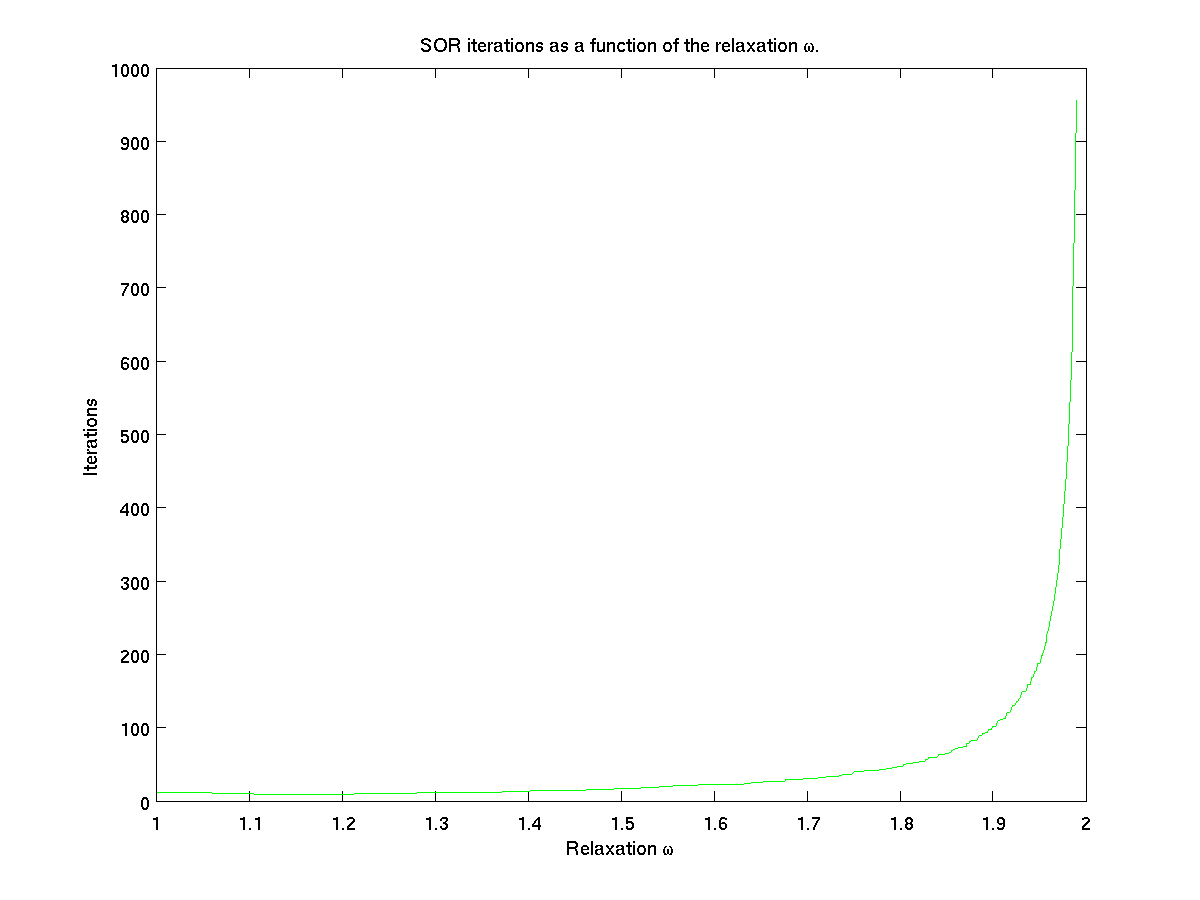
\includegraphics[width=\linewidth]{../img/task6_plot.png}
\else
	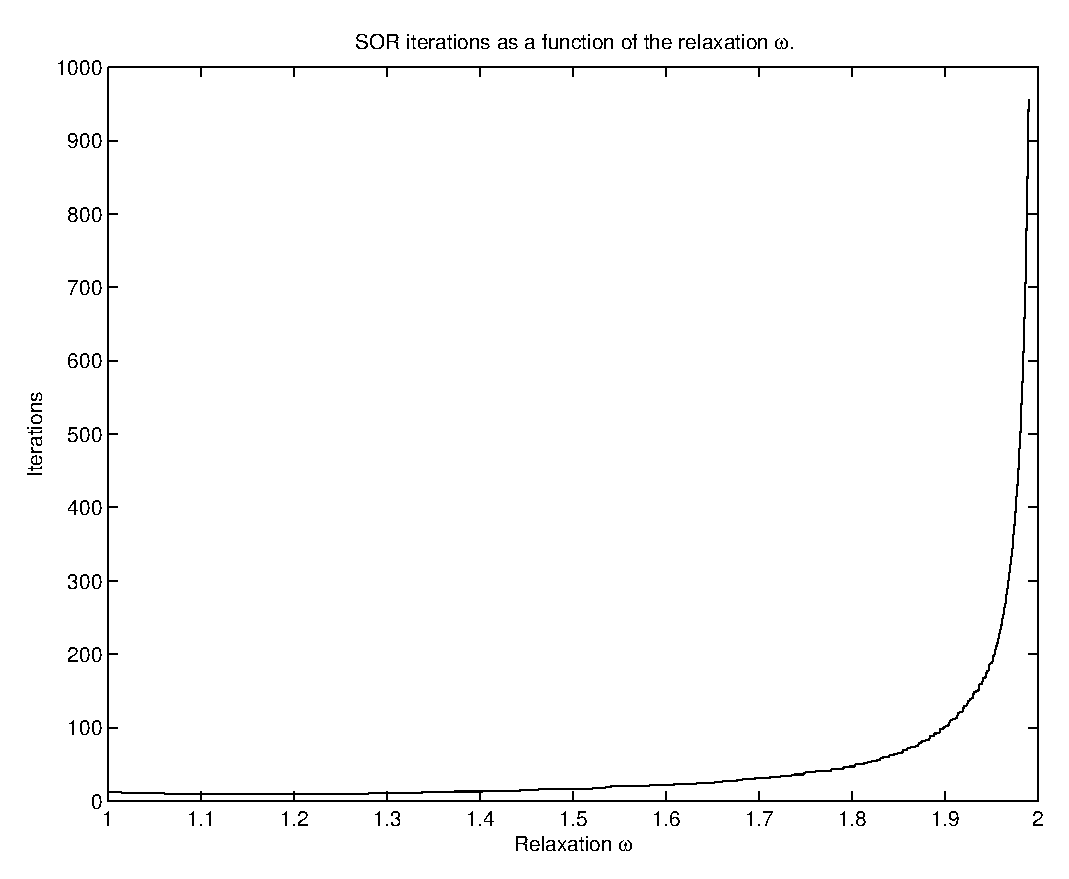
\includegraphics[width=\linewidth]{../img/task6_plot.eps}
\fi
\end{center}
\label{fig+task6}
\caption{}
\end{figure}

\subsection{Task \#7}
Running for $5$ hours SOR was able to solve systems with $2^{13}$ unknowns. This is better then the naive GE probalby since it finds solution that are only correct to the 4th decimal. However it is much slower than GE using \matlab{}s backslash operator. This hints about the sprase structure not being fully exploited here.

\subsection{Task \#8}
Mathematically it is the same equation being solved but using the backslash operator is more efficient than multiplying with the inverse because at each iteration step we have the matrix $\omega L + D$ which is a lower triangluar sprase matrix and the backslash operator sees this and can optimize using only forward substitution instread of the costly matrix multiplication.

After this change was made the script for task \#7 was now showed that SOR could solve systems with $2^{22}$ unknowns. This is the same number as in task \#5 where the backslash operator also was used. Thus the SOR implementation is now more efficient!

\subsection{Task \#10}
With $n=8$ and $100$ time measurements, the mean time for solving the original system ($A\times x=b$) with naive Gaussian elimination is $0.008563$ seconds  and for the perturbed system ($A_p\times x=b_p$) $0.008500$ seconds (i.e. $99.26\%$ of the original mean time). We see that there is almost no difference in solving a slightly different system.

\subsection{Task \#11}
With $n=8$ and $100$ time measurements, the mean time for solving the original system ($Ax=b$) with SOR (in Fixed-Point Iteration mode) is $0.003601$ seconds and for the perturbed system ($A_p\times x=b_p$) $0.001449$ seconds (i.e. $40.23\%$ of the original mean time). We see that it is possible to solve slight different system iteratively with SOR very efficient if we can exploit solutions to an slight different system. This is very useful in real time applications such as signal processing because the sample rate is so high that not much will change from each sample to the next.

Lets compare the results with the one found previously for GE.

\begin{eqnarray}
	\frac{\mathrm{mean}_{\mathrm{SOR, orig}}}{\mathrm{mean}_{\mathrm{GE, orig}}}=\frac{0.003601}{0.008563} & =42.053\% \\ \nonumber
	\frac{\mathrm{mean}_{\mathrm{SOR, pert}}}{\mathrm{mean}_{\mathrm{GE, pert}}}=\frac{0.001449}{0.008500} & =17.047\% \nonumber
\end{eqnarray}

We see that SOR is much better; especially for a perturbed system.

\subsection{Task \#12}
When redoing the previous two tasks but increasing k as much as posible it turns out that for GE $2^7$ systems could be measured 100 times to get average times for the original as $13.95055$ seconds and for the perturbed $13.94964$ seconds (i.e $\frac{Pert}{Orig}=99.99\%$ of the original mean.) For SOR it was $2^{21}$ and $14.77553$ seconds for the original system and $7.76254$ seconds for the perturbed (i.e. $\frac{Pert}{Orig}=52.54\%$ of the original mean). These k:s ($log_2()$) of the system size) represent how large systems we can have when we want to measure the average solve time $100$ times for GE and SOR as will be done in the next exercise. The best n, the one that works for both GE and SOR, is $n=2^7$.


\subsection{Task \#13}
The results from running both GE and SOR $100$ times for $8$ perturbed systems are shown in table \ref{table+avgpert}. We see that the total means does not deviate so much from the mean times found in task $\#12$. The only thing I notes is the 7th perturbed system solved with SOR that had an average notworty lower than the rests. I belive that the discrepancy is caused by the fact that the \matlab{} process is running on a shared system where the OS decides what processes will get execution time. 


%What is more intreressting is to ask if these results were the expected. If we assume that the execution time for the functions are linear we would from task $\#10$ and $\#11$ expect the average mean times to be:
%\begin{displaymath}
	%\mathrm{mean}_{GE,k=2^7}=\mathrm{mean}_{GE,k=2^3}\times2^{7-3}\times8=0.008500\times2^7=1.
%\end {displaymath}

Redoing the calculations from task $\#11$ gives:
\begin{displaymath}
	\frac{\mathrm{mean}_{\mathrm{SOR, pert}}}{\mathrm{mean}_{\mathrm{GE, pert}}}=\frac{7.0320083050}{13.8909941537} = 50.623\% % TODO new numbers for SOR.
\end{displaymath}

\begin{table}[h]
\begin{center}
\begin{tabular}{l l | l}
\multicolumn{2}{r}{GE [s]} & SOR [s]  \\ \cline{2-3} % TODO insert new results for SOR.
		& 13.9126260200 & 7.6632646200 \\
		& 13.8981966600 & 7.3282680400 \\
		& 13.8661602900 & 7.1929892400 \\
		& 13.9028463100 & 7.1854961600 \\
		& 13.8716484400 & 7.0341115700 \\
		& 13.9065633500 & 7.2155508300 \\
		& 13.8556906300 & 5.4708077500 \\
		& 13.9142215300 & 7.1655782300 \\ \cline{2-3}
Total mean	& 13.8909941537 & 7.0320083050 
\end{tabular}
\caption{Average times when solving 8 perturbed systems 100 times each.}
\end{center}
\label{table+avgpert}
\end{table}

\section{Lessons Learned}
From this project several theoretical understandings are gained.
\begin{itemize}
	\item Successive Over-Relaxation
	\item Sparse matrices  and how it affects numerical analysis.
	\item Benefits of using iterative methods on large systems that does not deviate much from a system with a known solution.
	\item 
\end{itemize}

In this project I've learned a lot about \matlab{}. It has been used in numerous coursed for Computer Scientist at LTH but not in any course have we really learned how to use it. After this project I really feel that I know how to use. This course or one including learning \matlab{} should have been included early in the education and not in the third year. More specifically:

\begin{itemize}
	\item I feel more comfortable in using the data types.
	\item Language control structures.
	\item How to use and write functions properly.
	\item Exception handling.
	\item Formatted strings.
	\item Execution time measurements.
	\item Running scripts as batch jobs.
	\item Using sparse matrices.
	\item Global and persistent variables.
	\item Many other details \ldots
\end{itemize}


\section{Acknowledgments}
I first implemented all tasks my self. Then I discussed the results with friends and adjusted some small things.

In exercise 3 in this course I, Gustaf Waldemarson and Erik Jansson implemented a simpler version of SOR. I used this as the basis for the SOR implementation in this project.

With Tommy Ivarsson, Oscar Olsson and Tommy Olsson I discussed the stopping criteria for SOR. With the first Tommy I also discussed the results found in task $\#13$.

\bibliography{references}{}
\bibliographystyle{ieeetr}

\newpage
\section*{Appendix}
\appendix
\section{Program listings} \label{appendix+programs}
Here the \matlab{} functions and scripts used to achieve the results above are listed.

\subsection{Scripts}
The following scrips are the drivers for producing the results found in this report.

\lstinputlisting{../src/task2.m}
\lstinputlisting{../src/task3.m}
\lstinputlisting{../src/task4.m}
\lstinputlisting{../src/task5.m}
\lstinputlisting[literate={∈}{$\in$}1]{../src/task6.m} % Replace the malformed UTF8 sequence with the LaTeX equivalent.
\lstinputlisting{../src/task7.m}
\lstinputlisting{../src/task9.m}
\lstinputlisting{../src/task10.m}
\lstinputlisting{../src/task11.m}
\lstinputlisting{../src/task12.m}
\lstinputlisting{../src/task13.m}

\subsection{Functions}
The following functions implements the algorithms and the rest serves as helper functions to these algorithms and the scripts. To distinguish these from other \matlab{}-functions in the global namespace these reside in a own package called \emph{pr1}.

\lstinputlisting{../src/+pr1/init_task.m}
\lstinputlisting{../src/+pr1/make_mat.m}
\lstinputlisting{../src/+pr1/make_perturbed_mat.m}
\lstinputlisting{../src/+pr1/naive_gauss.m}
\lstinputlisting{../src/+pr1/duosolve_gauss.m}
\lstinputlisting{../src/+pr1/multi_solve_gauss.m}
\lstinputlisting{../src/+pr1/sor.m}
\lstinputlisting{../src/+pr1/duosolve_sor.m}
\lstinputlisting{../src/+pr1/multi_solve_sor.m}
\lstinputlisting{../src/+pr1/time_out.m}

\end{document}
